\documentclass[withoutpreface,bwprint]{cumcmthesis} %去掉封面与编号页,电子版提交的时候使用。

\usepackage[framemethod=TikZ]{mdframed}
\usepackage{url}   % 网页链接
\usepackage{subcaption} % 子标题
\usepackage{mathtools}

\bibliographystyle{plain}

\title{“FAST”主动反射面的形状调节}
\begin{document}

\maketitle
\begin{abstract}
    我就是一個簡單的摘要。我还不到下一行吗???我就要到下一行了吧,太好了,嘿嘿嘿。下一行,我来了!
    我就是在下一行。
    \keywords{关键词1\quad 鬼哭狼嚎\quad 无人生还}
\end{abstract}

%目录  2019 明确不要目录,我觉得这个规定太好了
%\tableofcontents

%\newpage

\section{问题重述}
中国天眼——$500$米口径球面射电望远镜(Five-hundred-meter Aperture Spherical radio
Telescope,简称 FAST),是我国具有自主知识产权的目前世界上单口径最大、灵敏度最高的
射电望远镜。它的落成启用,对我国在科学前沿实现重大原创突破、加快创新驱动发展具有重
要意义。

FAST 由主动反射面、信号接收系统(馈源舱)以及相关的控制、测量和支承系统组成,其中
主动反射面系统是由主索网、反射面板、下拉索、促动器及支承结构等主要部件构成的一个可
调节球面。主索网由柔性主索按照短程线三角网格方式构成,用于支承反射面板(含背架结
构),每个三角网格上安装一块反射面板,整个索网固定在周边支承结构上。每个主索节点连
接一根下拉索,下拉索下端与固定在地表的促动器连接,实现对主索网的形态控制。反射面板
间有一定缝隙,能够确保反射面板在变位时不会被挤压、拉扯而变形。

主动反射面可分为两个状态:基准态和工作态。基准态时反射面为半径约 $300$ 米、口径为
$500$ 米的球面(基准球面);工作态时反射面的形状被调节为一个 $300$ 米口径的近似旋转抛物
面(工作抛物面)。馈源舱接收平面的中心只能在与基准球面同心的一个球面(焦面)上移动,两同
心球面的半径差为 F=$0.466$R(其中 R 为基准球面半径,称 F/R 为焦径比)。馈源舱接收信号
的有效区域为直径 $1$ 米的中心圆盘。当 FAST 观测某个方向的天体目标时,馈源舱接收平面的中
心被移动到天体目标与基准球面的球心连成的直线与焦面的交点处,调节基准球面上的部分反射面板
形成以天体目标与基准球面的球心连成的直线为对称轴、以馈源舱接收信号为焦点的近似旋转
抛物面,从而将来自目标天体的平行电磁波反射汇聚到馈源舱的有效区域。

将反射面调节为工作抛物面是主动反射面技术的关键,该过程通过下拉索与促动器配合来
完成。下拉索长度固定。促动器沿基准球面径向安装,其底端固定在地面,顶端可沿基准球面
径向伸缩来完成下拉索的调节,从而调节反射面板的位置,最终形成工作抛物面。

本赛题要解决的问题是:在反射面板调节约束下,确定一个理想抛物面,然后通过调节促
动器的径向伸缩量,将反射面调节为工作抛物面,使得该工作抛物面尽量贴近理想抛物面,以
获得天体电磁波经反射面反射后的最佳接收效果。

请你们团队根据附录中的要求及相关参数建立模型解决以下问题:
\begin{enumerate}
    \item 当待观测天体 $𝑆$ 位于基准球面正上方,即 $\alpha = 0°$, $\beta = 90°$ 时,结合考虑反
          射面板调节因素,确定理想抛物面。
    \item 当待观测天体 $𝑆$ 位于 $\alpha = 36.795°$, $\beta = 78.169°$ 时,确定理想抛物面。
          建立反射面板调节模型,调节相关促动器的伸缩量,使反射面尽量贴近该理想抛物面。将理想抛物面
          的顶点坐标,以及调节后反射面 $300$ 米口径内的主索节点编号、位置坐标、各促动器的伸缩量等
          结果按照规定的格式(见附件 $4$)保存在“result.xlsx”文件中。
    \item 基于第 $2$ 问的反射面调节方案,计算调节后馈源舱的接收比,即馈源舱有效区域接收到
          的反射信号与 $300$ 米口径内反射面的反射信号之比,并与基准反射球面的接收比作比较。
\end{enumerate}

\section{问题分析}
对于问题一,由于理想抛物面的对称性,我们可以将原先的三维问题看为一个二维问题。我们以球心为原点建立
直角坐标系,再设出理想抛物面的一个平面上的方程,与反射面板向上伸缩至极限时的方程联立,得到交点的坐标。
再结合反射面板的调节限制,进行枚举,得到最合适的理想抛物面的解。
\section{模型建立}
\subsection{符号说明}
\begin{center}
    \begin{tabular}{cc}
        \hline
        \makebox[0.3\textwidth][c]{符号} & \makebox[0.4\textwidth][c]{意义} \\
        \hline
        D                                & 木条宽度(cm)                   \\
        \hline
    \end{tabular}
\end{center}
\subsection{问题一}
\subsubsection{模型的建立}
由于理想抛物面和基准球面对 $z$ 轴对称,所以我们考虑只截取其中一个平面,建立一个平面直角坐标系。
以基准球面的球心为原点,建立如图 \ref{fig:coordinate1} 所示的直角坐标系。
\begin{figure}[!h]
    \centering
    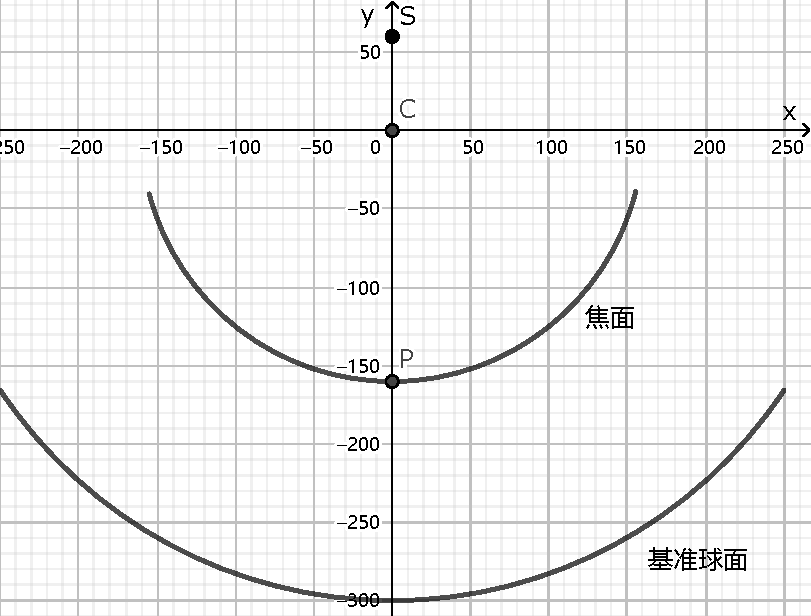
\includegraphics[width=.45\textwidth]{CoordinateSystem1.pdf}
    \caption{坐标系示意图}
    \label{fig:coordinate1}
\end{figure}
坐标系中基准球面的方程为 $x^2 + y^2 = 300^2$。反射面板向下伸缩至极限时的方程为
$x^2 + y^2 = (300 + 0.6)^2$,向上伸缩至极限时的方程为 $x^2 + y^2 = (300 - 0.6)^2$。

设理想抛物面在此平面上投影的方程为 $x^2 = 4p(y + a)$,将其与反射板向上伸缩至极限时的方程联立
\[
    \begin{dcases}
        x^2 = 4p(y + a) \\
        x^2 + y^2 = (300 - 0.6)^2
    \end{dcases}
\]
解得
\[
    \text{\huge $x =$}
    \begin{dcases}
        -\sqrt{\frac{4\,{\left(5\,a-801\right)}\,{\left(2\,\sqrt{\frac{41295363226730493}
        {34359738368}-4005\,a}-5\,a+1602\right)}}{25}}                    \\
        -\sqrt{-\frac{4\,{\left(5\,a-801\right)}\,{\left(5\,a+2\,\sqrt{
        \frac{41295363226730493}{34359738368}-4005\,a}-1602\right)}}{25}} \\
        \sqrt{\frac{4\,{\left(5\,a-801\right)}\,{\left(2\,\sqrt{\frac{41295363226730493}
        {34359738368}-4005\,a}-5\,a+1602\right)}}{25}}                    \\
        \sqrt{-\frac{4\,{\left(5\,a-801\right)}\,{\left(5\,a+2\,\sqrt{
        \frac{41295363226730493}{34359738368}-4005\,a}-1602\right)}}{25}}
    \end{dcases}
\]
其中 $a$ 的范围为 $[300 - 0.6, 300 + 0.6]$
\subsubsection{模型的解}
在 $a$ 的取值范围内对 $a$ 进行枚举,得出最优值。
\nocite{宋叶志2019}
\bibliography{references}
\begin{appendices}
    附录的内容。。。
\end{appendices}
\end{document}